\documentclass{article}

\usepackage{mystyle}
\usepackage{myvars}

%-----------------------------

\begin{document}

  \maketitle

  \part{Ejercicios Montgomery:}

  \setcounter{section}{2}
  \subsection{En la tabla B.1 del apéndice aparecen datos sobre el desempeño de los 26 equipos de la Liga Nacional de Fútbol en 1976. Se cree que la cantidad de yardas ganadas por tierra por los contrarios ($x_8$) tiene un efecto sobre la cantidad de juegos que gana un equipo ($y$).}
  \subsubsection{Ajustar un modelo de regresión lineal simple que relacione los juegos ganados, $y$, con las yardas ganadas por tierra por los contrarios, $x_8$.}

  \begin{equation}
  \label{eq:simple-linear-regression-model}
    y_i = \beta_0 + \beta_1x_8_i + \varepsilon_i
  \end{equation}
  \paragraph{}
  Analizaremos el modelo de la ecuación \ref{eq:simple-linear-regression-model} mediante un estudio de regresión lineal simple, con $y$ como variable dependiente, $x_8$ como variable independiente, $\beta_0$ el intercepto, y $\beta_1$ la pendiente. $\varepsilon$ es el error aleatorio.

  \paragraph{}
  El procedimiento \textit{REG} permite estimar los valores del intercepto y la pendiente, y analizar las hipótesis nulas:

    \begin{align}
      H_0: \beta_0 = 0\\
      H_0': \beta_1 = 0
      \label{mont:hipotesisnulas}
    \end{align}

  \paragraph{}
  La hipótesis más importante en la regresión es la que incumbe a $\beta_1$, ya que si la pendiente de la recta es 0, no existe regresión, y se trata de una población simple sobre la que $x_8$ no tiene efecto.

  \begin{figure}[H]
    \centering
    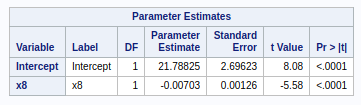
\includegraphics[width=.5\textwidth]{img/montgomery/procreg.png}
    \caption{Estimadores y p-valores para la regresión.}
    \label{img:mont-procreg}
  \end{figure}

  \paragraph{}
  Como podemos ver, el \textit{p-valor} para $\beta_1$ está por debajo de $0,05$, por lo que podemos rechazar la hipótesis nula con una confianza del 95\%. El \textit{p-valor} para el intercepto también permite rechazar la hipótesis nula.

  \paragraph{}
  Por tanto, los estimadores son:

  \begin{align}
    \hat\beta_0 = 21.78825\\
    \hat\beta_1 = -0.00703
  \end{align}

  \paragraph{}
  Con la recta de regresión:

  \begin{equation}
    y_i = 21.78825 -0.00703x_8_i + \varepsilon_i
  \end{equation}

  \paragraph{}
  La interpretación de estos parámetros es que con 0 yardas ganadas por el contrario, un equipo gana de media $21,78825$ juegos, y que por cada yarda que gana el contrario, el equipo pierde de media $0.00703$ juegos.

  \begin{figure}[H]
    \centering
    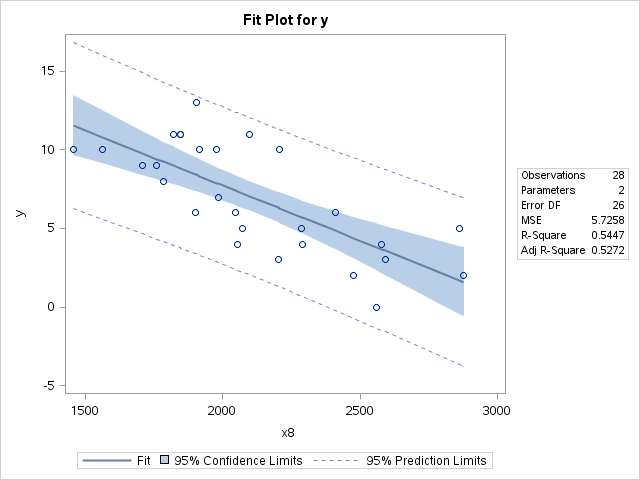
\includegraphics[width=.8\linewidth]{img/montgomery/fitplot.png}
    \caption{Fit plot del modelo de regresión lineal simple}
    \label{img:mont-fitplot}
  \end{figure}

  \subsubsection{Formar la tabla de análisis de varianza y probar el significado de la regresión.}

  \subsubsection{Determinar un intervalo de confianza de 95\% para la pendiente.}

  \subsubsection{¿Qué porcentaje de variabilidad total da $y$, y explica este modelo?}

  \subsubsection{Determinar un intervalo de confianza de 95\% para la cantidad promedio de juegos ganados, si la distancia ganada por tierra por los contrarios se limita a 2000 yardas.}

  \subsection{Supóngase que se quiere usar el modelo desarrollado en el problema 2.1 para pronosticar la cantidad de juegos que ganará un equipo si puede limitar los avances por tierra de sus contrarios a 1800 yardas. Determinar un estimado de punto de la cantidad de juegos ganados cuando $x_8=1800$. Determinar un intervalo de predicción de 90\% para la cantidad de juegos ganados.}

  \part{Código Fuente}


\end{document}
